\section{Problemas no controle corporal}

%%%%%%%%%%%%%%%%%%%%%%%%%%%%%%%%%%%%%%%%%%%%%%%%%%%%%%%%%%%%%%%%%%%%%%%%%%%%%%%%
%%%%%%%%%%%%%%%%%%%%%%%%%%%%%%%%%%%%%%%%%%%%%%%%%%%%%%%%%%%%%%%%%%%%%%%%%%%%%%%%
%%%%%%%%%%%%%%%%%%%%%%%%%%%%%%%%%%%%%%%%%%%%%%%%%%%%%%%%%%%%%%%%%%%%%%%%%%%%%%%%
\subsection{Dançar saltitando}
\index{Problemas!Saltitar}

\begin{problemT}[Saltitar quando dançamos:]
Eu percebo que o saltitar na dança das pessoas pode ter em alguns casos um origem mental e em outros um origem físico.
\begin{itemize}
\item \textbf{Mental:} Algumas vesses, o saltitar
é o jeito que  uma pessoa tem para conseguir acompanhar o pulso ou a métrica da música. 
Isto, quando a pessoa ainda não entende esses conceitos de forma conscientemente
e só percebe que quando saltita consegue acompanhar melhor a música.
\item \textbf{Físico:} Outras vezes o saltitar na dança pode ser devido a que a pessoa se movimenta na dança
com o peso do corpo dividido em ambos pés, de modo que quando deseja movimentar algum deles,
a pessoa tem muita dificuldade de tirar esse pé do chão; 
pois sem importar qual escolha na movimentação, a pessoa perderá o equilíbrio,
pelo que para movimentar-se o dançarino desenvolve o saltitar; quer dizer, 
ele faz um efeito mola nos joelhos ao igual que os dançarinos de ``swing'', 
para que no momento que estiquem os joelhos a pessoa tenha uma oportunidade de movimentar algum pé.    
\end{itemize}
\end{problemT}


\begin{SolutionT}[Relativa ao problema de saltitar:]
Para solucionar o saltitar na nossa dança devemos nos perguntar se o origem é mental, físico ou ambos;
neste sentido podemos ter em conta as seguintes recomendações:
\begin{itemize}
\item  Aprender a reconhecer os tempos fortes e os pulsos na música, 
libera à pessoa da necessidade de levar o pulso usando saltos.
Porém, mesmo depois de entender e identificar perfeitamente a métrica da música,
é possível que a pessoa ainda tenha o vicio de saltitar, mesmo que já não seja necessário;
neste caso a solução é identificar este vicio e segurar ele nas danças. Assim, 
nosso único foco de treinamento será não realizar estes saltos, ate perder essa costume.
\item  Realizaremos treinamentos atribuindo o peso do corpo a um pé 
antes de nos movimentar, primeiro sem acompanhamento musical,
e logo seguindo a música.
Este treinamento nos ajudará a ganhar a costume de ter o peso do corpo definido num pé,
antes de animar-nos a movimentar o outro. 
\end{itemize}
\end{SolutionT}




%%%%%%%%%%%%%%%%%%%%%%%%%%%%%%%%%%%%%%%%%%%%%%%%%%%%%%%%%%%%%%%%%%%%%%%%%%%%%%%%
%%%%%%%%%%%%%%%%%%%%%%%%%%%%%%%%%%%%%%%%%%%%%%%%%%%%%%%%%%%%%%%%%%%%%%%%%%%%%%%%
%%%%%%%%%%%%%%%%%%%%%%%%%%%%%%%%%%%%%%%%%%%%%%%%%%%%%%%%%%%%%%%%%%%%%%%%%%%%%%%%
\subsection{Errar no controle do corpo}
\index{Problemas!Controlar o corpo}



Tenho observado que algumas pessoas tem dificuldade
em realizar algum movimento simples explicado nas aulas de dança.
Entre os movimentos com dificuldade temos:
\begin{description}
\item[Movimento 1:] Ir em linha reta quando realizamos vários giros.
\textbf{Problema:} Temos um desvio no percorrido e realizamos uma linha curva e não uma reta.
\item[Movimento 2:] Ter os pés juntos quando realizamos o passo básico frente traz no samba de gafieira.
\textbf{Problema:} Por vicio, algumas pessoas fazem este movimento de forma hibrida com o passo básico do forró,
levando um pé atrás e não deixando eles juntos.\\
\end{description} 


\begin{figure}[!h]
\begin{elaboracion}{O utopista{,} o pessimista e o pragmático}
Quando uma pessoa se vê enfrentada a um problema, 
o qual não pode corrigir,
ou não se sente capaz de corrigir; ela pode adotar diferentes posturas:
\begin{description}
\item[A pessoa utopista] reconhece sua falência, mas persiste no caminho  escolhido
e que acha correto, pois é sonhadora com ideais quiméricas, 
e mesmo detetando um erro intrínseco nele, que lhe impede terminar uma tarefa,
continua persistindo sem se desviar do caminho.
No exemplo da figura, o otimista treina apontando a um alvo, 
mas todas as vesses erra o tiro com uma desviação que reconhece proveniente de um problema intrínseco nele;
porém, ele persiste, pois acha que um dia o desvio desaparecerá.
\item[A pessoa pessimista] reconhece sua falência, 
vê uma dificuldade intrínseca nele para realizar uma tarefa; aborda o problema pelo lado negativo,
concluindo que não será capaz de completar a tarefa.
No exemplo da figura, o pessimista reconhece sua dificuldade intrínseca em atingir o alvo
e desiste da tarefa. 
\item[A pessoa pragmática] reconhece sua falência, e se estas não podem ser corrigidas,
procura soluções práticas, realistas e objetivas, 
aceitando abordagens e soluções quase-ótimas ao problema.
No exemplo da figura, o pragmático reconhece a desviação,
 no seu senso de posição espacial, e não luta com a realidade; pelo contrario, se adapta a esta 
para obter a resposta desejada. 
\end{description}
\begin{center}
    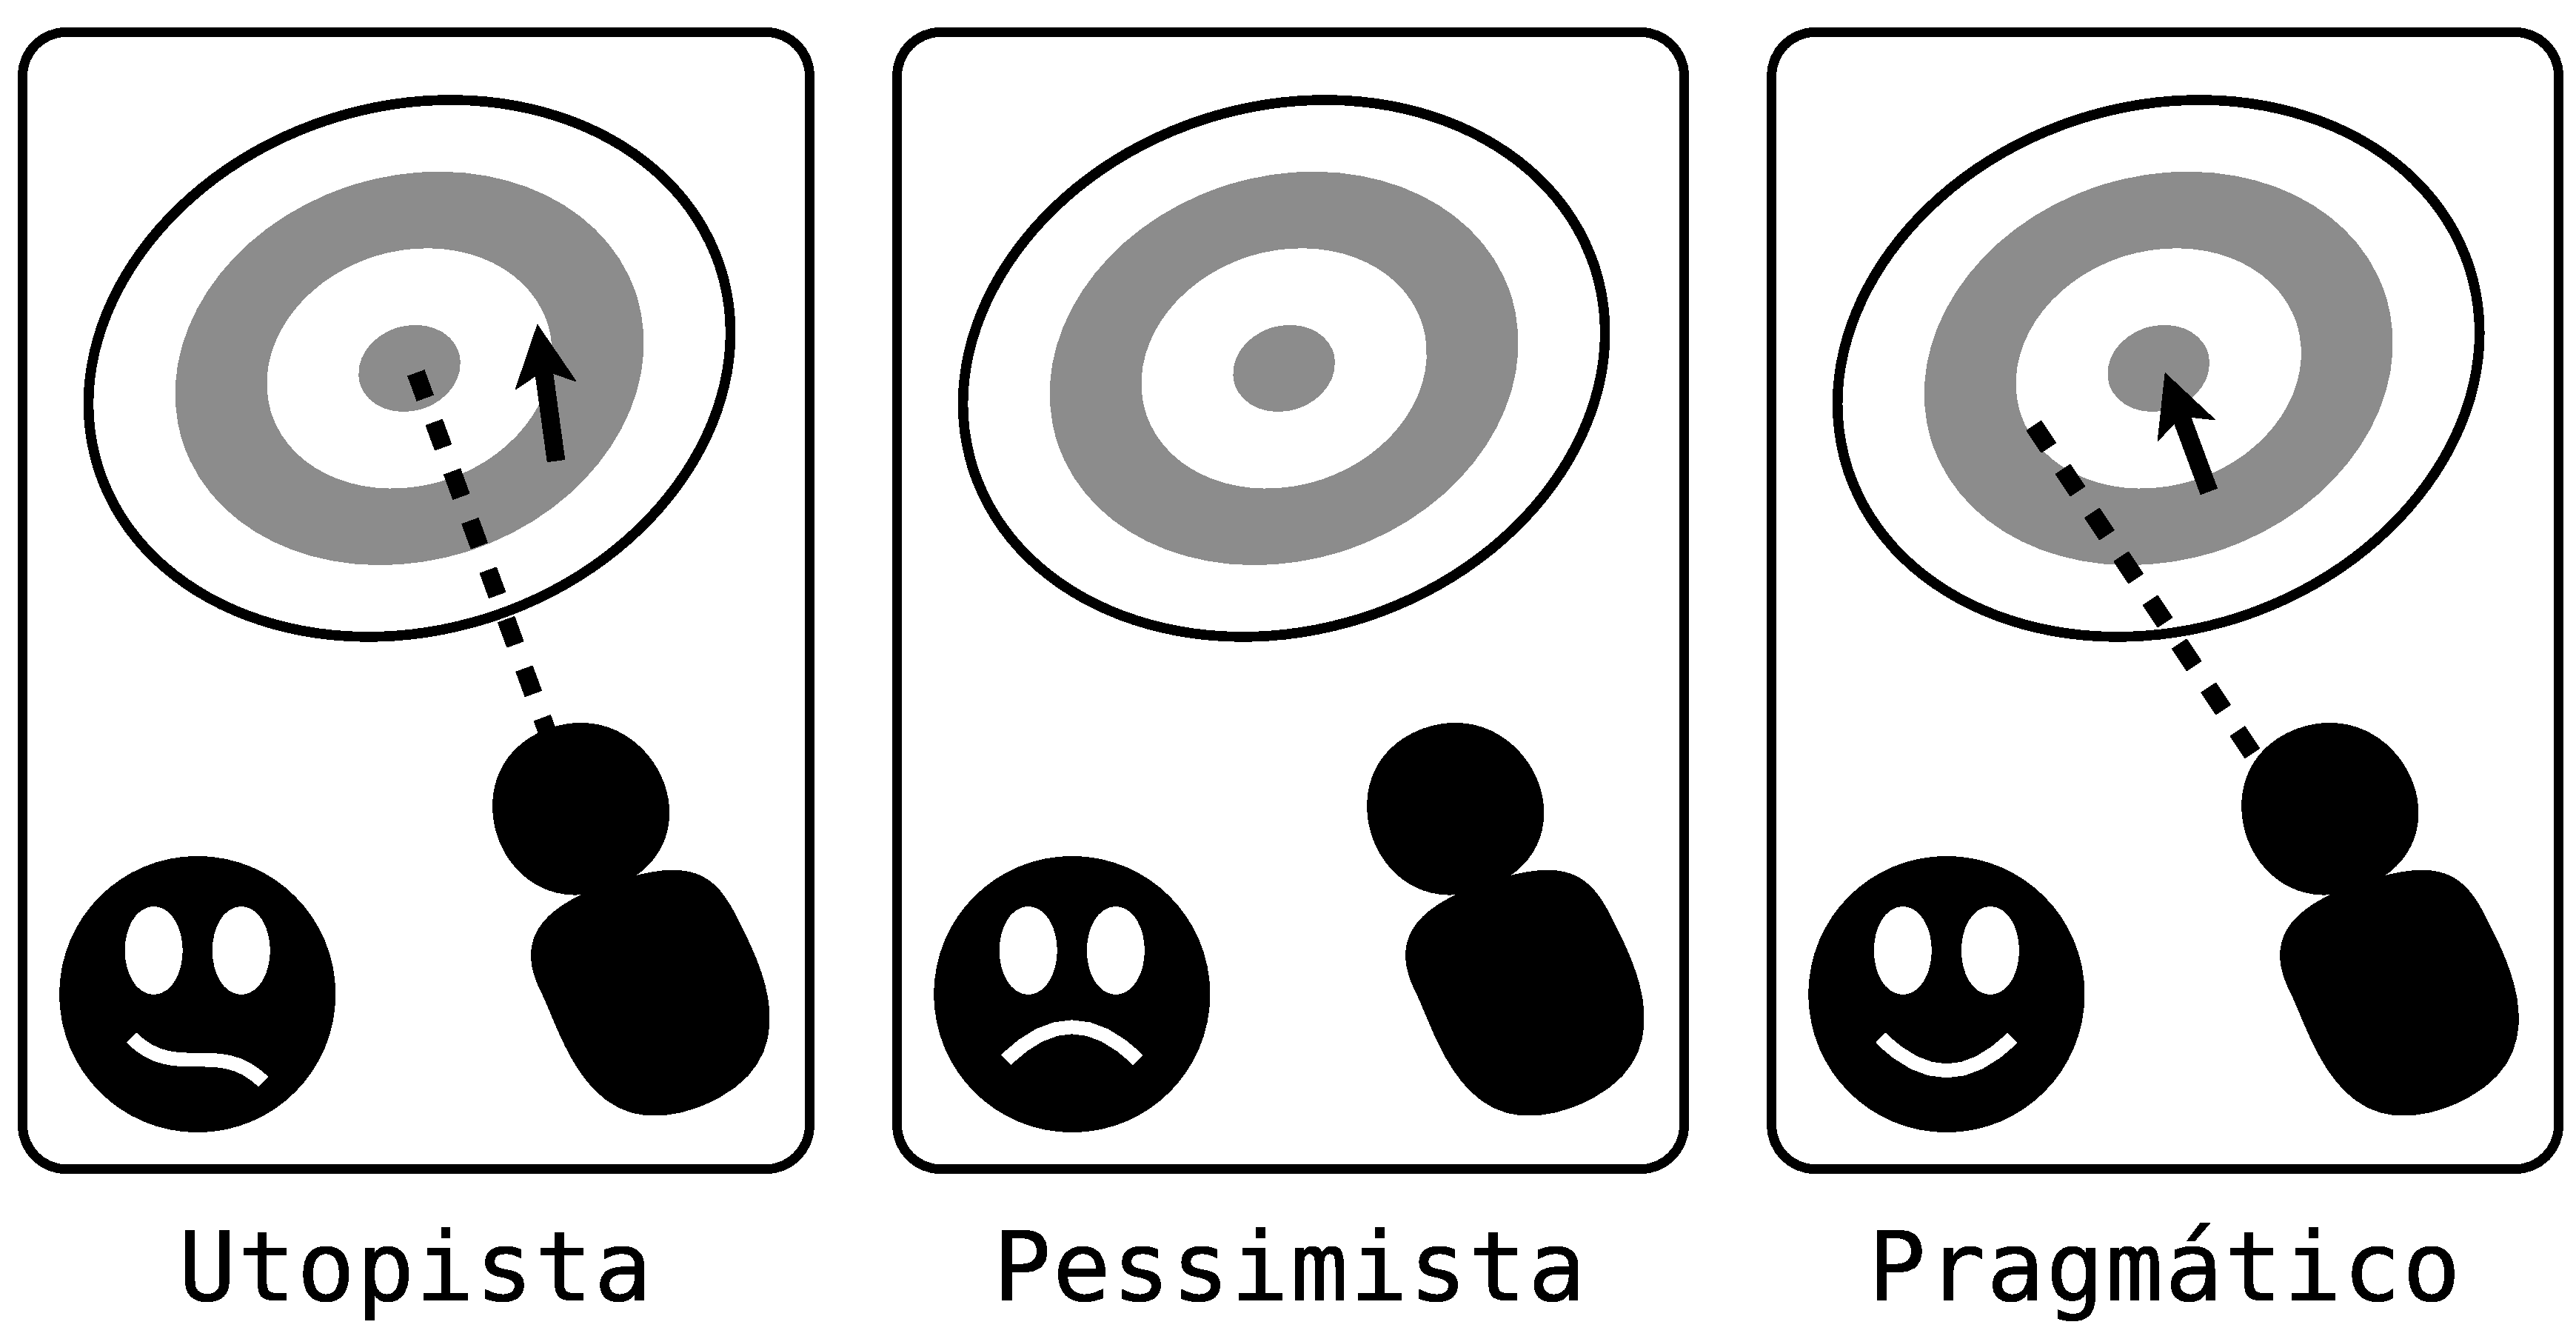
\includegraphics[width=0.7\textwidth]{chapters/cap-body-control/problema-generico-completo.eps}
\end{center}
\end{elaboracion}
\end{figure}


Mesmo que nestos casos poderíamos alegar que os problemas não são graves,
devemos prestar atenção que estes manifestam que a pessoa não tem conhecimento e domínio do seu corpo,
e isto pode impedir que a pessoa aprenda movimentos mais complexos,
pois ainda não tomou consciência da importância de conhecer seu próprio corpo para poder controlá-lo.
Nos casos anteriores é possível ter uma abordagem pragmática dos problemas.
Por exemplo:
\begin{description}
\item[Solução ao problema do movimento 1:] Se ao tentar em ir em linha reta, realizamos uma curva a esquerda,
em vez de tentar ir em linha reta, podemos tentar ter uma pequena desviação à direita,
ate que consigamos conferir que finalmente realizamos uma linha reta.
\item[Solução ao problema do movimento 2:] Se ao realizar um movimento de frente traz no samba de gafieira,
não podemos evitar colocar o pé direito atrás,
como quando dançamos forró; 
então uma solução seria deixar de tentar colocar ambos pés juntos,
e em cambio ordenar a nosso corpo colocar o pé direito ligeiramente adiantado,
ate perceber que na realidade colocamos os pés juntos.
\end{description} 


\begin{figure}[!ht]
\begin{elaboracion}{Ah\'i viene Mart\'in Corona (1952)}

A modo de anedota é interessante mencionar que esse desvio natural,
que as pessoas temos no nosso senso espacial, 
é muito conhecido desde antanho por pessoas pragmáticas;
por exemplo, podemos ver uma referencia a isto no filme ``Ahí viene Martín Corona'' (1952),
ambientado em México na época de vaqueiros, quatreiros e pistolas,
quando a personagem ``Piporro'', amigo da família de ``Martín'', 
apos perseguir e dar castigo aos assassinos dos pais do Martín, ainda criança, 
ensina a este a disparar.
O seguinte dialogo acontece aproximadamente aos 4 min. 15 seg. iniciado o filme.
\begin{description}
\item[Piporro:] 
Para ``pegar-lhe''\footnote{\label{foot:pegarle}Pegar-lhe: Atirar e atingir.} ao centro de um relógio, 
tem que lhe apontar abaxinho do 6. %\footnote{\label{foot:abaixinho}Abaixinho: Diminutivo de abaixo.}
Agora que se quer ``pegar-lhe''\footref{foot:pegarle} a um criminal na 
``mera''\footnote{\label{foot:mera}Mera | Mero: Palavra que serve para realçar; exatamente na.} frente, não tem perca,
aponta-lhe ao ``ocico''\footnote{\label{foot:ocico}Ocico: Focinho.}.
Agora que se trata-se de ``pegar-lhe''\footref{foot:pegarle} a 
um ``pelao''\footnote{\label{foot:pelao}Pelao: Pessoa grosseira, vulgar e inculta.} 
``fachoso''\footnote{\label{foot:fachoso}Fachoso: Desleixado excêntrico e extravagante.} no ``mero''\footref{foot:mera} coração,
escuta, segue este conselho, aponta-lhe ao umbigo.

\item[Martin:] Ao umbigo?

\item[Piporro:] Ao ``mero''\footref{foot:mera} umbigo! você que lhe aponta ai, ele que cai, sem dizer ai.
\end{description}
\end{elaboracion}
\end{figure}
